\documentclass[../Head/Main.tex]{subfiles}
\begin{document}
\section{Introduction}

The goal of the project is to develop a self-contained program in python to count the number of pumpkins in a drone camera capture.
During the development multiple algorithms and methods should be tested and evaluated in comparison.

The image we used can be seen in figure \ref{fig:DJI_0237}

\begin{figure}[H]
	\centering
	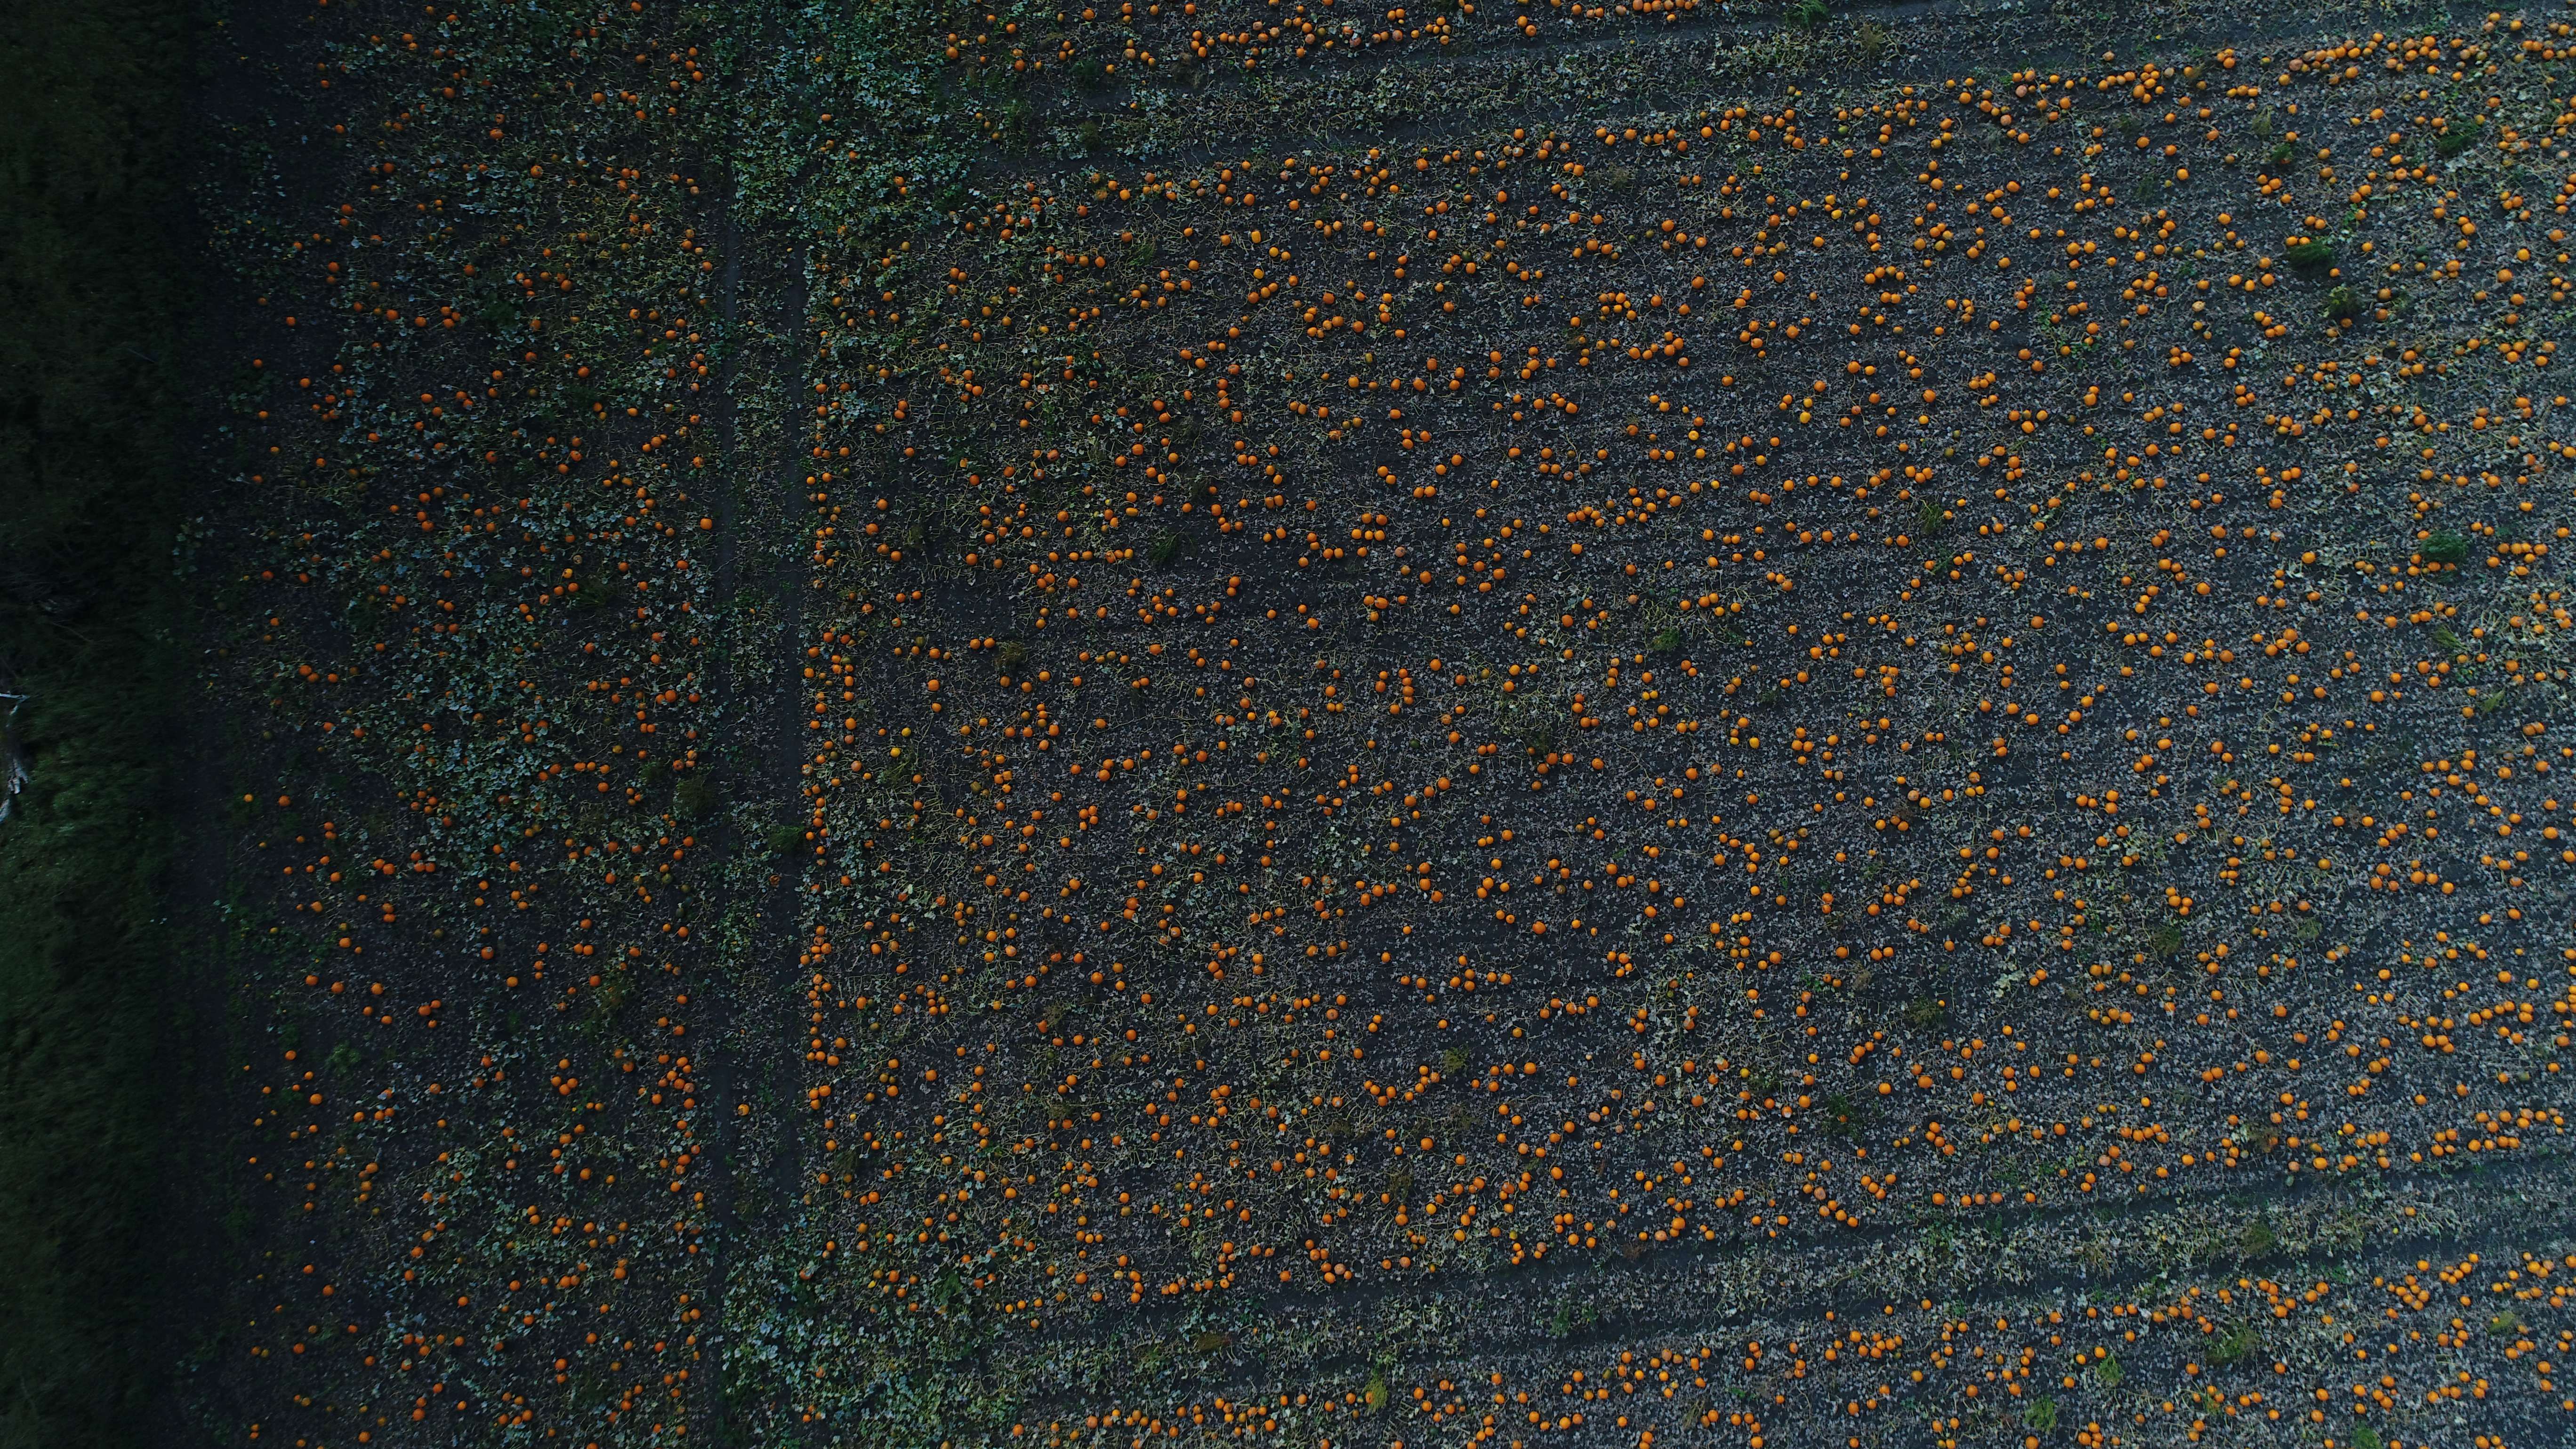
\includegraphics[width=0.75\textwidth]{../Figures/DJI_0237.JPG}
	\caption{DJI\_0237.JPG}
	\label{fig:DJI_0237}
\end{figure}


\end{document}